\documentclass[10pt,a4paper]{article}
\usepackage{fontspec}
\usepackage{amsmath}
\usepackage{amsfonts}
\usepackage{amssymb}
\usepackage{graphicx}
\usepackage[spanish,es-nodecimaldot]{babel}
\usepackage{subfigure}
\usepackage{natbib}
\usepackage[titletoc]{appendix}
\usepackage[hidelinks, unicode = true]{hyperref}
\author{José Ignacio Escribano}
\title{Superficies regladas}

%*******************************************************
%                 NO MODIFICAR
\newcommand*{\FSfont}[1]{%
  \fontencoding{T1}\fontfamily{#1}\selectfont}

\newlength{\tpheight}\setlength{\tpheight}{0.9\textheight}
\newlength{\txtheight}\setlength{\txtheight}{0.9\tpheight}
\newlength{\tpwidth}\setlength{\tpwidth}{0.9\textwidth}
\newlength{\txtwidth}\setlength{\txtwidth}{0.9\tpwidth}
\newlength{\drop}
%*******************************************************

% Crea una portada con los siguientes parámetros
%
% #1 : Título 
% #2 : Subtítulo
% #3 : Subsubtítulo
% #4 : Autor(es)
% #5 : Lugar
%

\newcommand*{\portada}[5]{
\begin{titlepage}
\begingroup
\vspace*{1cm}
\drop = 0.2\txtheight
\centering
\vfill
{\Huge \scshape #1}\\[\baselineskip]
{\Large \textbf{#2}}\\[\baselineskip]
{\Large \scshape #3}\\[\baselineskip]
\vspace*{0.3cm}
{\large \textit{#4}}\\[0.5\drop]

\includegraphics[scale=0.35]{./images/logoURJC.jpg}
\vspace*{1.5cm}

{\large \scshape #5, \today} \par
\begin{center}
\end{center}
\vfill\null
\endgroup
\end{titlepage}
}
 %*****************************************************
\usepackage{amsmath}
\usepackage{xparse}
\usepackage{amsthm}
\usepackage{tikz}

% Seno
\def\sen{\mathop{\mbox{\normalfont sen}}\nolimits}

% Seno hiperbólico
\def\senh{\mathop{\mbox{\normalfont senh}}\nolimits}

% Arcoseno
\def\arcsen{\mathop{\mbox{\normalfont arcsen}}\nolimits}

% Gradiente
\def\grad{\mathop{\mbox{\normalfont grad}}\nolimits}

% Argumento principal
\def\Arg{\mathop{\mbox{\normalfont Arg}}\nolimits}

% Logaritmo complejo
\def\Log{\mathop{\mbox{\normalfont Log}}\nolimits}

% Rotacional
\def\rot{\mathop{\mbox{\normalfont rot}}\nolimits}

% Divergencia
\def\diver{\mathop{\mbox{\normalfont div}}\nolimits}

% Longitud
\def\longi{\mathop{\mbox{\normalfont long}}\nolimits}

% Índice de una curva
\def\ind{\mathop{\mbox{\normalfont Ind}}\nolimits}

% Norma
\newcommand{\norm}[1]{\lVert #1 \rVert}

% Derivada parcial
\newcommand{\derpar}[1]{\dfrac{\partial}{\partial #1}}

% Derivada parcial con función
\newcommand{\derparcial}[2]{\dfrac{\partial #1}{\partial #2}}

% Derivada parcial de orden n con funcion
\newcommand{\derparcialn}[3]{\dfrac{\partial^{#3} #1}{\partial #2^{#3}}}

% Integral doble en [a,b] x [c,d]
\newcommand{\intdob}[4]{\displaystyle \int_{#1}^{#2} \int_{#3}^{#4}}

% Integral triple en [a,b] x [c,d] x [e,f]
\newcommand{\inttri}[6]{\displaystyle \int_{#1}^{#2} \int_{#3}^{#4} \int_{#5}^{#6}}

% Números complejos
\def\C{\ensuremath{\mathbb{C}}}

% Números reales
\def\R{\ensuremath{\mathbb{R}}}

% Números racionales
\def\Q{\ensuremath{\mathbb{Q}}}

% Números enteros
\def\Z{\ensuremath{\mathbb{Z}}}

% Números naturales
\def\N{\ensuremath{\mathbb{N}}}

% Teorema
\newtheorem{teo}{Teorema}

% Corolario
\newtheorem{cor}{Corolario}

% Proposición
\newtheorem{prop}{Proposición}

% Lema
\newtheorem{lema}{Lema}

% Definición
\newtheorem{defi}{Definición}

% Observaciones
\newtheorem*{obs}{Observaciones}

% Observación
\newtheorem*{ob}{Observación}

% Nota
\newtheorem*{nota}{Nota}

% Pregunta
\newtheorem*{pregunta}{Pregunta}

% Ejemplo
\newtheorem*{ejemplo}{Ejemplo}


\NewDocumentCommand{\overarrow}{O{=} O{\uparrow} m}{%
  \overset{\makebox[0pt]{\begin{tabular}{@{}c@{}}#3\\[0pt]\ensuremath{#2}\end{tabular}}}{#1}
}
\NewDocumentCommand{\underarrow}{O{=} O{\downarrow} m}{%
  \underset{\makebox[0pt]{\begin{tabular}{@{}c@{}}\ensuremath{#2}\\[0pt]#3\end{tabular}}}{\ensuremath{#1}}
}

\newcommand{\contradiction}{%
\begin{tikzpicture}[rotate=45,x=0.5ex,y=0.5ex]
\draw[color=red, line width=.1ex] (0,2) -- (3,2) (0,1) -- (3,1) (1,3) -- (1,0) (2,3) -- (2,0);
\end{tikzpicture}
}


\begin{document}
	
\portada{Superficies regladas}{ \ }{ \ }{José Ignacio Escribano (GIS + MAT)}{Móstoles}

\tableofcontents
\newpage

\listoffigures
\newpage

\section{Introducción}

Antes de comenzar a definir los conceptos básicos de superficies regladas, recordaremos la definición de superficie.

\begin{defi}
	Una superficie es una aplicación
	\begin{equation}
	r : [a,b] \times [c,d] \subseteq \R^2 \to \R^3
	\end{equation}
\end{defi}

Aunque existen definiciones más elaboradas de superficies para nuestros propósitos es suficiente.\\

Veamos algunos ejemplos de superficies:

\begin{ejemplo}[Esfera]
Uno de los ejemplos típicos de superficie es la esfera de radio $r$ (centrada en $(0,0,0)$) que viene dada por la aplicación siguiente:

$$\begin{array}{rcll}
	r : & [0, 2\pi] \times [-\pi/2, \pi/2] & \to & \R^3\\
		& (u,v) & \mapsto & (x(u,v), y(u,v), z(u,v))
\end{array}$$
		
donde 

$$\begin{cases}
x(u,v) = r\cos u \cos v \\
y(u,v) = r\sin u \cos v \\
z(u,v) = r\sen v
\end{cases}$$

La representación en Mathematica se puede ver en la Figura~\ref{fig:esfera}.

\begin{figure}[thbp]
	\centering
	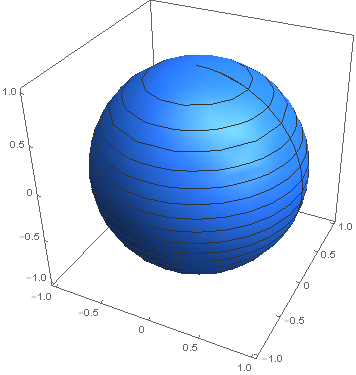
\includegraphics[width=0.5\linewidth]{../Imágenes/esfera}
	\caption{Esfera de radio $1$}
	\label{fig:esfera}
\end{figure}

\end{ejemplo}

\begin{ejemplo}[Plano]
Otro ejemplo típico de superficie es el plano que pasa por el punto $(x_0, y_0, z_0)$ y tiene por vectores directores a  $(w_1, w_2, w_3)$ y $(p_1, p_2, p_3)$, que puede parametrizarse con la aplicación siguiente:


$$\begin{array}{rcll}
	r : & \R^2 & \to & \R^3\\
		& (u,v) & \mapsto & (x(u,v), y(u,v), z(u,v))
\end{array}$$
		
donde 

$$\begin{cases}
x(u,v) = x_0 + w_1 u + p_1 v \\
y(u,v) = y_0 + w_2 u + p_2 v \\
z(u,v) = z_0 + w_3 u + p_3 v
\end{cases}$$

La representación en Mathematica se puede ver en la Figura~\ref{fig:plano}.

\begin{figure}[thbp]
	\centering
	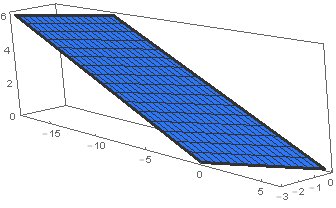
\includegraphics[width=0.5\linewidth]{../Imágenes/plano}
	\caption{Plano}
	\label{fig:plano}
\end{figure}

\end{ejemplo}

\begin{ejemplo}[Cilindro]
Por último consideraremos, el cilindro de radio $r$, que viene parametrizado por la siguiente aplicación:


$$\begin{array}{rcll}
	r : & [0, 2\pi] \times \R & \to & \R^3\\
		& (u,v) & \mapsto & (x(u,v), y(u,v), z(u,v))
\end{array}$$
		
donde 

$$\begin{cases}
x(u,v) = r \cos u  \\
y(u,v) = r \sen u \\
z(u,v) = v
\end{cases}$$

La representación en Mathematica se puede ver en la Figura~\ref{fig:cilindro}.

\begin{figure}[thbp]
	\centering
	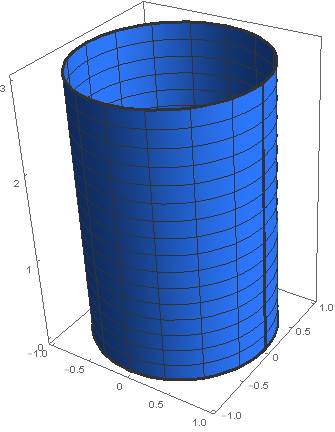
\includegraphics[width=0.3\linewidth]{../Imágenes/cilindro}
	\caption{Plano}
	\label{fig:cilindro}
\end{figure}

\end{ejemplo}

\subsection{Superficies regladas}

La idea de una superficie reglada es que puede ser generada por una recta en el espacio.

\begin{defi}
Una superficie reglada es aquella generada por una recta en el espacio llamada generatriz, a lo largo de una curva llamada directriz.\\

La parametrización de una superficie reglada es 
			
\begin{equation}
r(u,v) = \rho(u) + v a(u)
\end{equation}

donde $\rho, a : I = [a,b] \to \R^3$ son dos curvas en el espacio.
\end{defi}

Algunos tipos de superficies regladas son las superficies cilíndricas, superficies cónicas, las superficies de Catalan o los conoides.

\begin{defi}
	Una superficie reglada es cilíndrica si es de la forma 
	
	\begin{equation}
	r(u,v) = \rho(u) + v a_0
	\end{equation}
	
	con $a_0 \in \R^3$.
\end{defi}

\begin{defi}
	Una superficie reglada es cónica si es de la forma 
	
	\begin{equation}
	r(u,v) = \rho_0 + v a(u)
	\end{equation}
	
	con $\rho_0 \in \R^3$.\\
	
	$\rho_0$ es el vértice del cono.
\end{defi}

\begin{defi}
	Una superficie reglada es tangente desarrollable si es de la forma 
	
	\begin{equation}
	r(u,v) = \rho(u) + v \rho'(u)
	\end{equation}
\end{defi}

\begin{defi}
	Una superficie reglada que cumple que $a'(u) \neq 0 \ \ \forall u \in I$ se denomina no cilíndrica. 
\end{defi}

\begin{defi}
	Una superficie no cilíndrica cuyas generatrices son paralelas a un plano directriz fijo se llama superficie de Catalan.
\end{defi}

\begin{teo}[Caracterización de las superficies de Catalan]
	Una superficie reglada $r(u,v) = \rho(u) + v a(u)$ es una superficie de Catalan si y sólo si
	\begin{equation}
	[a(u), a'(a), a''(u)] = 0,  a''(u) \neq 0 \ \ \forall u \in I
	\end{equation}
\end{teo}

\begin{defi}
	Una superficie de Catalan se dice conoide si todas las generatrices intersecan una recta constante (el eje del conoide).
\end{defi}

\begin{defi}
	Una superficie reglada se dice que es doblemente reglada si existen dos rectas que generan la superficie.
\end{defi}

\section{Algunas superficies regladas}

\subsection{Superficies cilíndricas y cónicas}

\begin{ejemplo}[Superficie cilíndrica y cónica]
Supongamos que queremos generar un cilindro y un cono a partir de una curva (ver Figura~\ref{fig:rosa-4-petalos}) dada por la siguiente parametrización:

$$\begin{array}{rcll}
	a : & [0, 2\pi] & \to & \R^2\\
		& t & \mapsto & (x(t), y(t))
\end{array}$$
		
donde 

$$ \begin{cases}
x(t) = \cos(2t)\cos t \\
y(t) = \cos(2t) \sen t
\end{cases} $$ 
	
\begin{figure}[htbp]
	\centering
	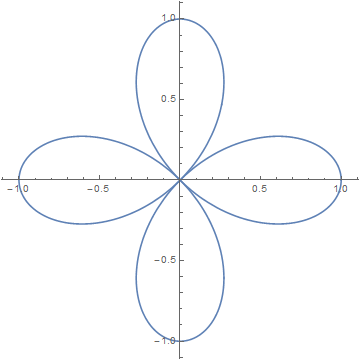
\includegraphics[width=0.5\linewidth]{../Imágenes/rosa-4-petalos}
	\caption{Rosa de cuatro pétalos}
	\label{fig:rosa-4-petalos}
\end{figure}

Comencemos con generando la superficie cilíndrica. Para ello, debemos fijar un punto $a_0$. En nuestro caso será el punto $(0,0,1)$. Con esto, una superficie cónica queda de la siguiente manera:

$$ r(u,v) = (\cos(2u)\cos u, \cos(2u) \sen u, v) $$

La Figura~\ref{fig:cilindro-rosa-4-petalos} muestra la superficie cilíndrica obtenida a partir de la curva. 

\begin{figure}
	\centering
	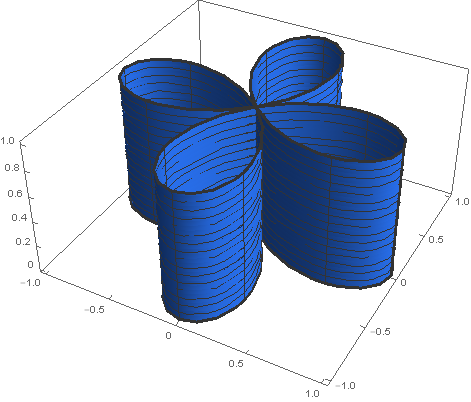
\includegraphics[width=0.5\linewidth]{../Imágenes/cilindro-rosa-4-petalos}
	\caption{Superficie cilíndrica a partir de la rosa de cuatro pétalos}
	\label{fig:cilindro-rosa-4-petalos}
\end{figure}

Para obtener la superficie cónica, fijamos $\rho_0 = (0,0,1)$. De esta manera obtenemos la superficie con parametrización siguiente

$$ r(u,v) = (v\cos(2u)\cos u, v\cos(2u)\sen u,v) $$ 

La Figura~\ref{fig:cono-rosa-4-petalos} muestra superficie cónica obtenida a partir de la curva.

\begin{figure}[htbp]
	\centering
	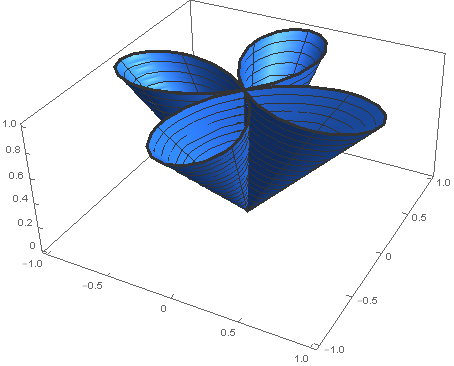
\includegraphics[width=0.5\linewidth]{../Imágenes/cono-rosa-4-petalos}
	\caption{Superficie cónica a partir de la rosa de cuatro pétalos}
	\label{fig:cono-rosa-4-petalos}
\end{figure}

\end{ejemplo}

\subsection{Conoide de Wallis}

\begin{defi}
El conoide de Wallis viene dado por la siguiente parametrización:

$$\begin{array}{rcll}
r : & [0, 2\pi] \times [0,1] & \to & \R^3\\
& (u,v) & \mapsto & (x(u,v),y(u,v),z(u,v))
\end{array}$$

donde 

$$ \begin{cases}
x(u,v) = v \cos u \\
y(u,v) = v \sen u \\
z(u,v) = c \sqrt{a^2 - b^2 \cos^2 u}
\end{cases} $$

donde $a, b, c \in \R$.
\end{defi}

La Figura~\ref{fig:conoide-de-Wallis-1} muestra el conoide de Wallis con $a = b = c = 1$.

\begin{figure}[htbp]
	\centering
	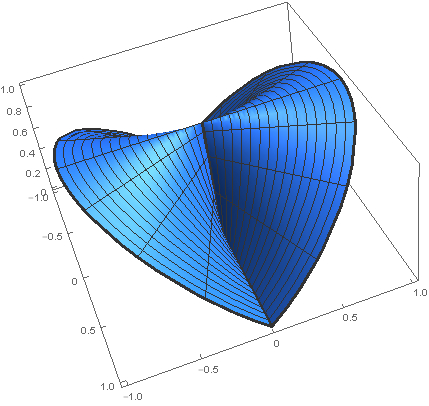
\includegraphics[width=0.5\linewidth]{../Imágenes/conoide-de-Wallis-1}
	\caption{Conoide de Wallis con $a=b=c=1$}
	\label{fig:conoide-de-Wallis-1}
\end{figure}

\begin{ejemplo}
Comprobemos que el conoide de Wallis es una superficie de Catalan. Para ello escribimos $r(u,v)$ de la siguiente forma para poder aplicar el teorema de caracterización de las superficies de Catalan:

$$ r(u,v) = (v\cos u, v\sen u, c\sqrt{a^2 - b^2 \cos^2 u}) = (0,0,c\sqrt{a^2 - b^2 \cos^2 u}) + v(\cos u, \sen u, 0) = \rho(u) + v a(u) $$

Calculamos la primera y la segunda derivada de $a$:

\begin{eqnarray*}
a'(u)  = &(-\sen u, \cos u, 0)\\
a''(u) = & (-\cos u, -\sen u, 0)
\end{eqnarray*}

Calculamos el producto mixto de $a(u), a'(u)$ y $a''(u)$,

$$ \left| \begin{array}{ccc}
\cos u & \sen u & 0 \\
-\sen u & \cos u & 0 \\
-\cos u & -\sen u & 0
\end{array} \right| = 0 $$

Además se cumple que $a''(u) \neq 0$ para todo $u \in [0, 2\pi]$ puesto que seno y coseno no se anulan simultáneamente.\\

Por tanto, el conoide de Wallis es una superficie de Catalan.

\end{ejemplo}


\subsection{Conoide de Plücker}

\begin{defi}
El conoide de Plücker es una superficie reglada dada por la siguiente parametrización: 

$$\begin{array}{rcll}
r : & [0, 2\pi] \times [0,1] & \to & \R^3\\
& (u,v) & \mapsto & (x(u,v),y(u,v),z(u,v))
\end{array}$$

donde 

$$ \begin{cases}
x(u,v) = v \cos u \\
y(u,v) = v \sen u \\
z(u,v) = \sen 2u
\end{cases} $$
\end{defi}

La Figura~\ref{fig:conoide-de-Plucker-1} muestra el conoide de Plücker

\begin{figure}
	\centering
	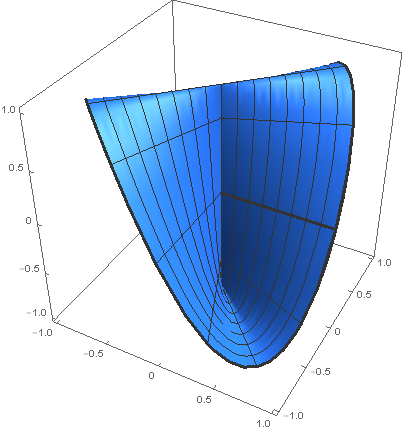
\includegraphics[width=0.5\linewidth]{../Imágenes/conoide-de-Plucker-n=2-1}
	\caption{Conoide de Plücker}
	\label{fig:conoide-de-Plucker-1}
\end{figure}

\subsection{Conoide de Plücker generalizado}

Existe una generalización del conoide de Plücker que describimos a continuación:

\begin{defi}
El conoide de Plücker generalizado viene dado por la siguiente parametrización:

$$\begin{array}{rcll}
r : & [0, 2\pi] \times [0,1] & \to & \R^3\\
& (u,v) & \mapsto & (x(u,v),y(u,v),z(u,v))
\end{array}$$

donde 

$$ \begin{cases}
x(u,v) = v \cos u \\
y(u,v) = v \sen u \\
z(u,v) = \sen nu
\end{cases} $$

\end{defi}

En efecto se trata de una generalización del conoide de Plücker visto anteriormente, poniendo $n = 2$.\\

La Figura~\ref{fig:plucker-generalizado} muestra dos conoides de Plücker generalizados, con $n = 2$ y $n = 5$, respectivamente.

\begin{figure}[htbp]
\centering
\subfigure[Conoide de Plücker generalizado con $n=3$]{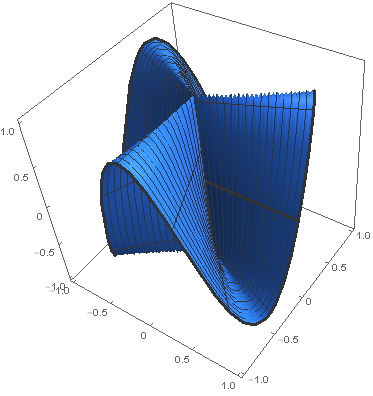
\includegraphics[width=0.5\linewidth]{../Imágenes/conoide-de-Plucker-n=3-1}}
\subfigure[Conoide de Plücker generalizado con $n=5$]{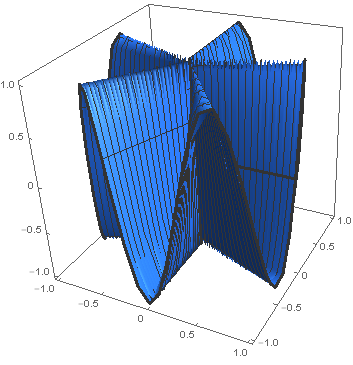
\includegraphics[width=0.5\linewidth]{../Imágenes/conoide-de-Plucker-n=5}}
\caption{Conoide de Plücker generalizado} \label{fig:plucker-generalizado}
\end{figure}

\begin{ejemplo}
Comprobemos que el conoide de Plücker es una superficie de Catalan. Escribimos $r(u,v)$ de la siguiente forma:

$$ r(u,v) = (0,0, \sen nu) + v(\cos u, \sen u, 0) = \rho(u) + v a(u) $$

Calculando las derivadas y el producto mixto se obtiene que es nulo para todo $u \in [0, 2 \pi]$ y que $a''(u) \neq 0 $ para todo $u \in [0, 2 \pi]$.

\end{ejemplo}

\subsection{Paraguas de Whitney}

\begin{defi}
El paraguas de Whitney es una superficie regular que tiene la siguiente parametrización:

$$\begin{array}{rcll}
r : & [-1, 1]^2 & \to & \R^3\\
& (u,v) & \mapsto & (x(u,v),y(u,v,z(u,v))
\end{array}$$

donde 

$$ \begin{cases}
x(u,v) = uv \\
y(u,v) = u \\
z(u,v) = v^2
\end{cases} $$
\end{defi}

La Figura~\ref{fig:paraguas-de-Whitney-1} muestra el paraguas de Whitney.

\begin{figure}[htbp]
	\centering
	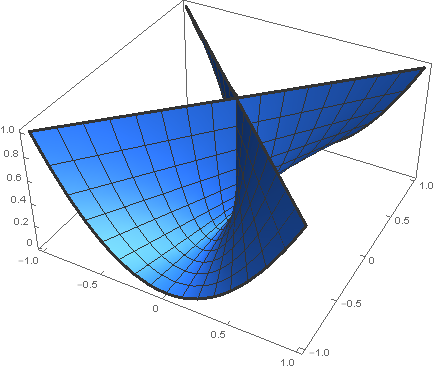
\includegraphics[width=0.5\linewidth]{../Imágenes/paraguas-de-whitney-1}
	\caption{Paraguas de Whitney}
	\label{fig:paraguas-de-Whitney-1}
\end{figure}

\subsection{Banda de Möbius}

\begin{defi}
La banda de Möbius viene dada por la parametrización siguiente:

$$\begin{array}{rcll}
r : & [0, 2\pi] \times [-1,1] & \to & \R^3\\
& (u,v) & \mapsto & (x(u,v),y(u,v),z(u,v))
\end{array}$$

donde 

$$ \begin{cases}
x(u,v) = \left( 1 + \frac{v}{2}\cos\frac{u}{2} \right)\cos u \\
y(u,v) = \left( 1 + \frac{v}{2}\cos\frac{u}{2} \right)\sen u \\
z(u,v) = \frac{v}{2}\sen\frac{u}{2}
\end{cases} $$
\end{defi}

La Figura~\ref{fig:banda-de-moebius} muestra la banda de Möbius.

\begin{figure}[htbp]
\centering
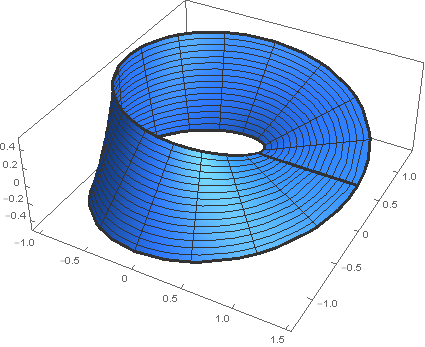
\includegraphics[width=0.5\linewidth]{../Imágenes/banda-de-moebius}
\caption{Banda de Möbius}
\label{fig:banda-de-moebius}
\end{figure}

\subsection{Helicoide}

\begin{defi}
El helicoide viene por la siguiente parametrización:

$$\begin{array}{rcll}
r : & [0, 2\pi] \times \R & \to & \R^3\\
& (u,v) & \mapsto & (x(u,v),y(u,v),z(u,v))
\end{array}$$

donde 

$$ \begin{cases}
x(u,v) = v\cos u \\
y(u,v) = v\sen u \\
z(u,v) = u
\end{cases} $$
\end{defi}

La Figura~\ref{fig:helicoide} muestra una representación del helicoide.

\begin{figure}[hbtp]
	\centering
	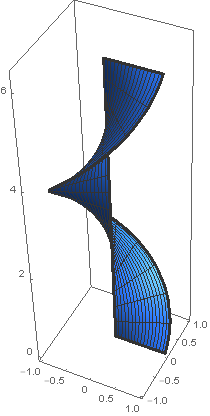
\includegraphics[width=0.3\linewidth]{../Imágenes/helicoide}
	\caption{Helicoide}
	\label{fig:helicoide}
\end{figure}

\subsection{Hiperboloide}

\begin{defi}

El hiperboloide es una superficie doblemente reglada que se puede parametrizar de la siguiente manera:

$$\begin{array}{rcll}
r : & \R \times [0, 2\pi] & \to & \R^3\\
& (u,v) & \mapsto & (x(u,v),y(u,v),z(u,v))
\end{array}$$

donde 

$$ \begin{cases}
x(u,v) = a \cosh u \cos v \\
y(u,v) = b \cosh u \sen v \\
z(u,v) = c \senh u
\end{cases} $$

donde $a, b, c \in \R$.

\end{defi}

La Figura~\ref{fig:hiperboloide} muestra la representación de un hiperboloide con $a = b = c = 1$.

\begin{figure}[htbp]
	\centering
	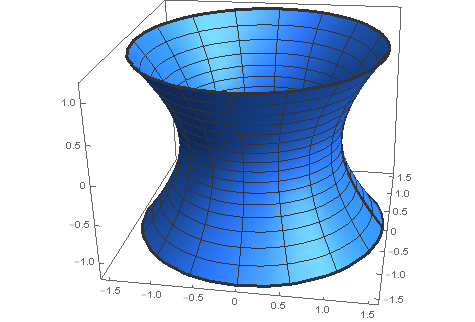
\includegraphics[width=0.5\linewidth]{../Imágenes/hiperboloide}
	\caption{Hiperboloide con $a=b=c=1$}
	\label{fig:hiperboloide}
\end{figure}

La parametrización anterior no se puede poner de la forma $r(u,v) = \rho(u) + v a(u)$, por lo que no sería una superficie reglada. Sin embargo, existen parametrizaciones del hiperboloide de la forma anterior:

\begin{defi}
El hiperboloide puede parametrizarse de las siguientes maneras:

$$\begin{array}{rcll}
r : & [0, 2\pi] \times \R & \to & \R^3\\
& (u,v) & \mapsto & (x(u,v),y(u,v),z(u,v))
\end{array}$$

donde 

$$ \begin{cases}
x(u,v) = a \cos u \mp av\cos u \\
y(u,v) = b \cos u \pm bv\sen u \\
z(u,v) = \pm c v
\end{cases} $$

donde $a, b, c \in \R$.

\end{defi}

Como existen dos parametrizaciones distintas de la forma $\rho(u) + v a(u)$, el hiperboloide se trata de una superficie doblemente reglada.

\subsection{Paraboloide hiperbólico}

\begin{defi}
	
El paraboloide hiperbólico es una superficie doblemente reglada que está dada por las parametrizaciones siguientes:

$$\begin{array}{rcll}
r : & \R^2 & \to & \R^3\\
& (u,v) & \mapsto & (x(u,v),y(u,v),z(u,v))
\end{array}$$

donde 

$$ \begin{cases}
x(u,v) = a(u+v) \\
y(u,v) = \pm bv \\
z(u,v) = u^2 +2uv
\end{cases} $$
\end{defi}

La Figura~\ref{fig:Paraboloide hiperbólico-2} muestra un paraboloide hiperbólico con $a = b = 1$.

\begin{figure}[htbp]
	\centering
	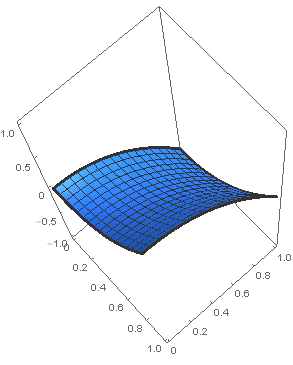
\includegraphics[width=0.8\linewidth]{../Imágenes/paraboloide-hiperbolico}
	\caption{Paraboloide hiperbólico con $a = b = 1$}
	\label{fig:Paraboloide hiperbólico-2}
\end{figure}

\subsection{Cola de milano}

\begin{defi}
La cola de milano (o Swallowtail) es una superficie reglada con la siguiente parametrización:

$$\begin{array}{rcll}
	r : & [-1, 1] \times [-2,2] & \to & \R^3\\
	& (u,v) & \mapsto & (x(u,v),y(u,v),z(u,v))
	\end{array}$$
	
	donde 
	
	$$ \begin{cases}
	x(u,v) = v \\
	y(u,v) = -4u^3 - 2uv \\
	z(u,v) = 3u^4 + u^2v
	\end{cases} $$
\end{defi}

La Figura~\ref{fig:cola-de-milano-1} muestra la cola de milano.\\

\begin{figure}
	\centering
	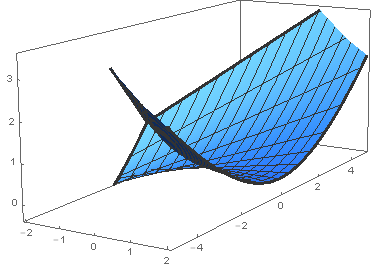
\includegraphics[width=0.5\linewidth]{../Imágenes/cola-de-milano-1}
	\caption{Cola de milano}
	\label{fig:cola-de-milano-1}
\end{figure}

Esta superficie inspiró a Salvador Dalí para su último cuadro, The Swallow's Tail, pintado en 1983.

\begin{figure}[htbp]
	\centering
	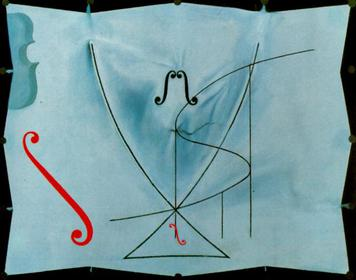
\includegraphics[width=0.5\linewidth]{../Imágenes/Aplicaciones/The_Swallowtail}
 	\caption[The Swallow's Tail]{The Swallow's Tail, Salvador Dalí \url{http://en.wikipedia.org/wiki/File:The\_Swallowtail.jpg}}
	\label{fig:dali}
\end{figure}

\section{Aplicaciones a la arquitectura}

Entre las muchas aplicaciones en las que se aplican las superficies regladas, una de las más importantes es la arquitectura donde se han aplicado en numerosas ocasiones. Veamos algunos ejemplos.\\

Se han aplicado superficies cónicas y cilíndricas en numerosas ocasiones como en la Escuela de la Sagrada Familia o en otros edificios como iglesias (Figura~\ref{fig:conos-y-cilindros})

\begin{figure}[htbp]
\centering
\subfigure[Techo de la Escuela de la Sagrada Familia. \url{http://en.wikipedia.org/wiki/File:Escuelas_Sagrada_Familia.jpg}]{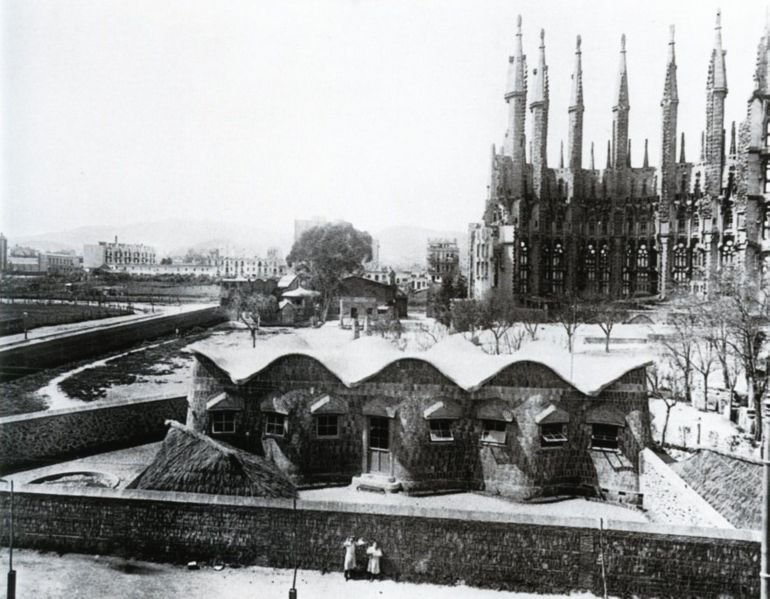
\includegraphics[width=0.5\linewidth]{../Imágenes/Aplicaciones/Escuelas_Sagrada_Familia}}
\subfigure[Iglesia en Selo, Eslovenia
\url{http://en.wikipedia.org/wiki/File:Nagytotlak.JPG}]{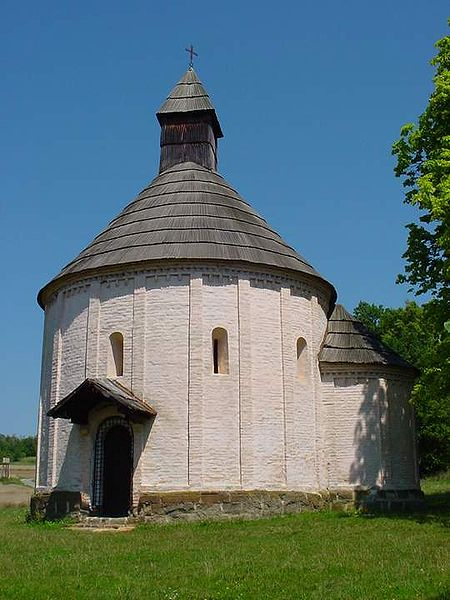
\includegraphics[width=0.35\linewidth]{../Imágenes/Aplicaciones/Nagytotlak}}
\caption{Superficies cónicas y cilíndricas en la arquitectura} \label{fig:conos-y-cilindros}
\end{figure}

También se han empleado en numerosas estructuras hiperbólicas en torres de refrigeración de centrales nucleares o distintas torres (Figura \ref{fig:hiperbolicos}).\\

\begin{figure}[htbp]
\centering
\subfigure[Torre de refrigeración en Didcot, Reino Unido \url{http://en.wikipedia.org/wiki/File:Didcot_power_station_cooling_tower_zootalures.jpg}]{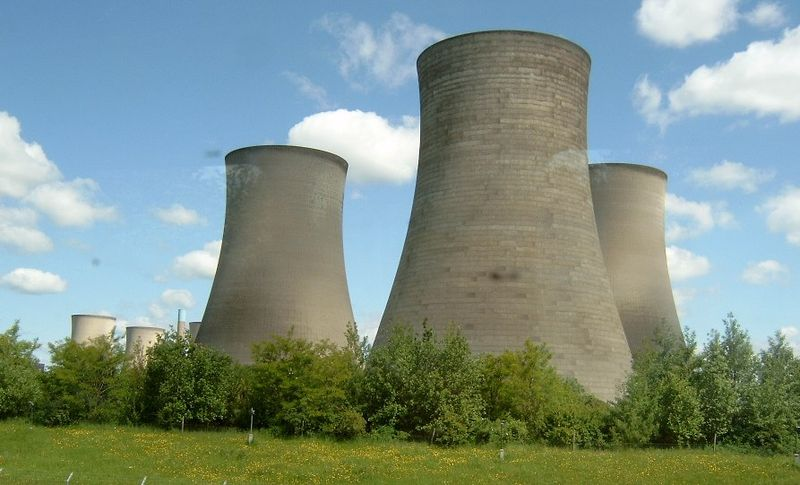
\includegraphics[width=0.4\linewidth]{../Imágenes/Aplicaciones/Didcot_power_station_cooling_tower_zootalures}}

\subfigure[Torre de agua en Ciechanów, Polonia \url{http://en.wikipedia.org/wiki/File:Ciechanow_water_tower.jpg}]{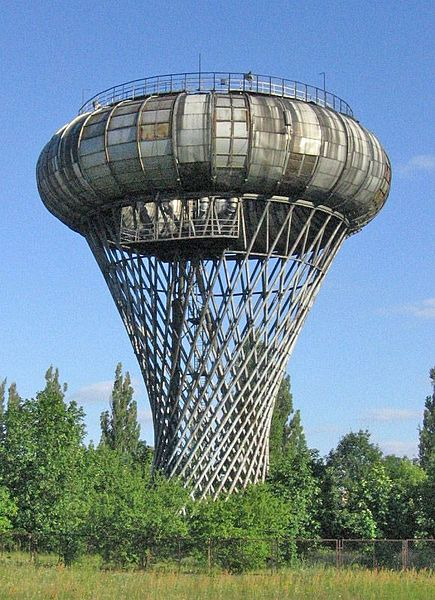
\includegraphics[width=0.35\linewidth]{../Imágenes/Aplicaciones/Ciechanow_water_tower}}

\subfigure[Torre del puerto en Kobe, Japón \url{http://en.wikipedia.org/wiki/File:Kobe_port_tower11s3200.jpg}]{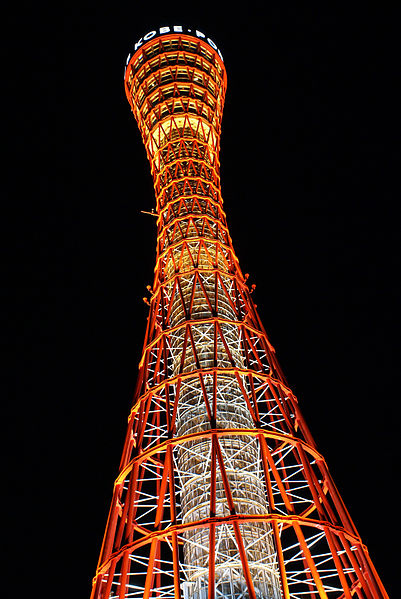
\includegraphics[width=0.35\linewidth]{../Imágenes/Aplicaciones/Kobe_port_tower11s3200}}

\caption{Superficies hiperbólicas en la arquitectura} \label{fig:hiperbolicos}
\end{figure}

Los paraboloides hiperbólicos se han utilizado en numerosos edificios, como estadios o estaciones de ferrocarriles (Figura~\ref{fig:paraboloides-hiperbolicos}).\\

\begin{figure}[htbp]
\centering
\subfigure[Techo de la estación de ferrocarriles de Ochota en Varsovia, Polonia
	\url{http://en.wikipedia.org/wiki/File:W-wa_Ochota_PKP-WKD.jpg}]{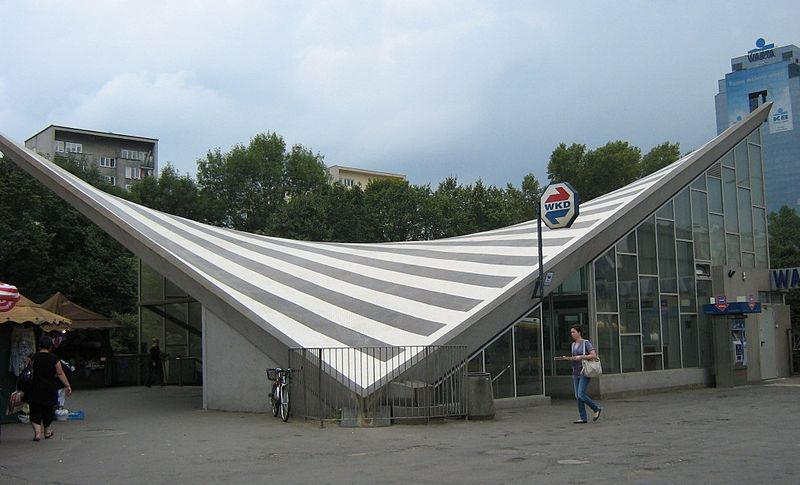
\includegraphics[width=0.6\linewidth]{../Imágenes/Aplicaciones/W-wa_Ochota_PKP-WKD}}

\subfigure[Scotiabank Saddledome en Calgary, Canadá
	\url{http://en.wikipedia.org/wiki/File:Pengrowth_Saddledome.jpg}]{	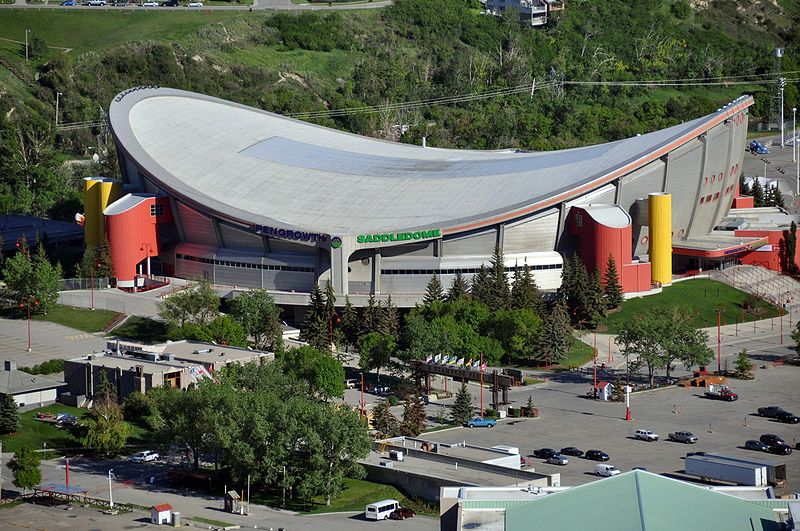
\includegraphics[width=0.5\linewidth]{../Imágenes/Aplicaciones/Pengrowth_Saddledome}}

\caption{Paraboloides hiperbólicos en la arquitectura} \label{fig:paraboloides-hiperbolicos}
\end{figure}

Por últimos, los helicoides se han utilizado para escaleras (Figura~\ref{fig:italia}).
 
\begin{figure}[htbp]
	\centering
	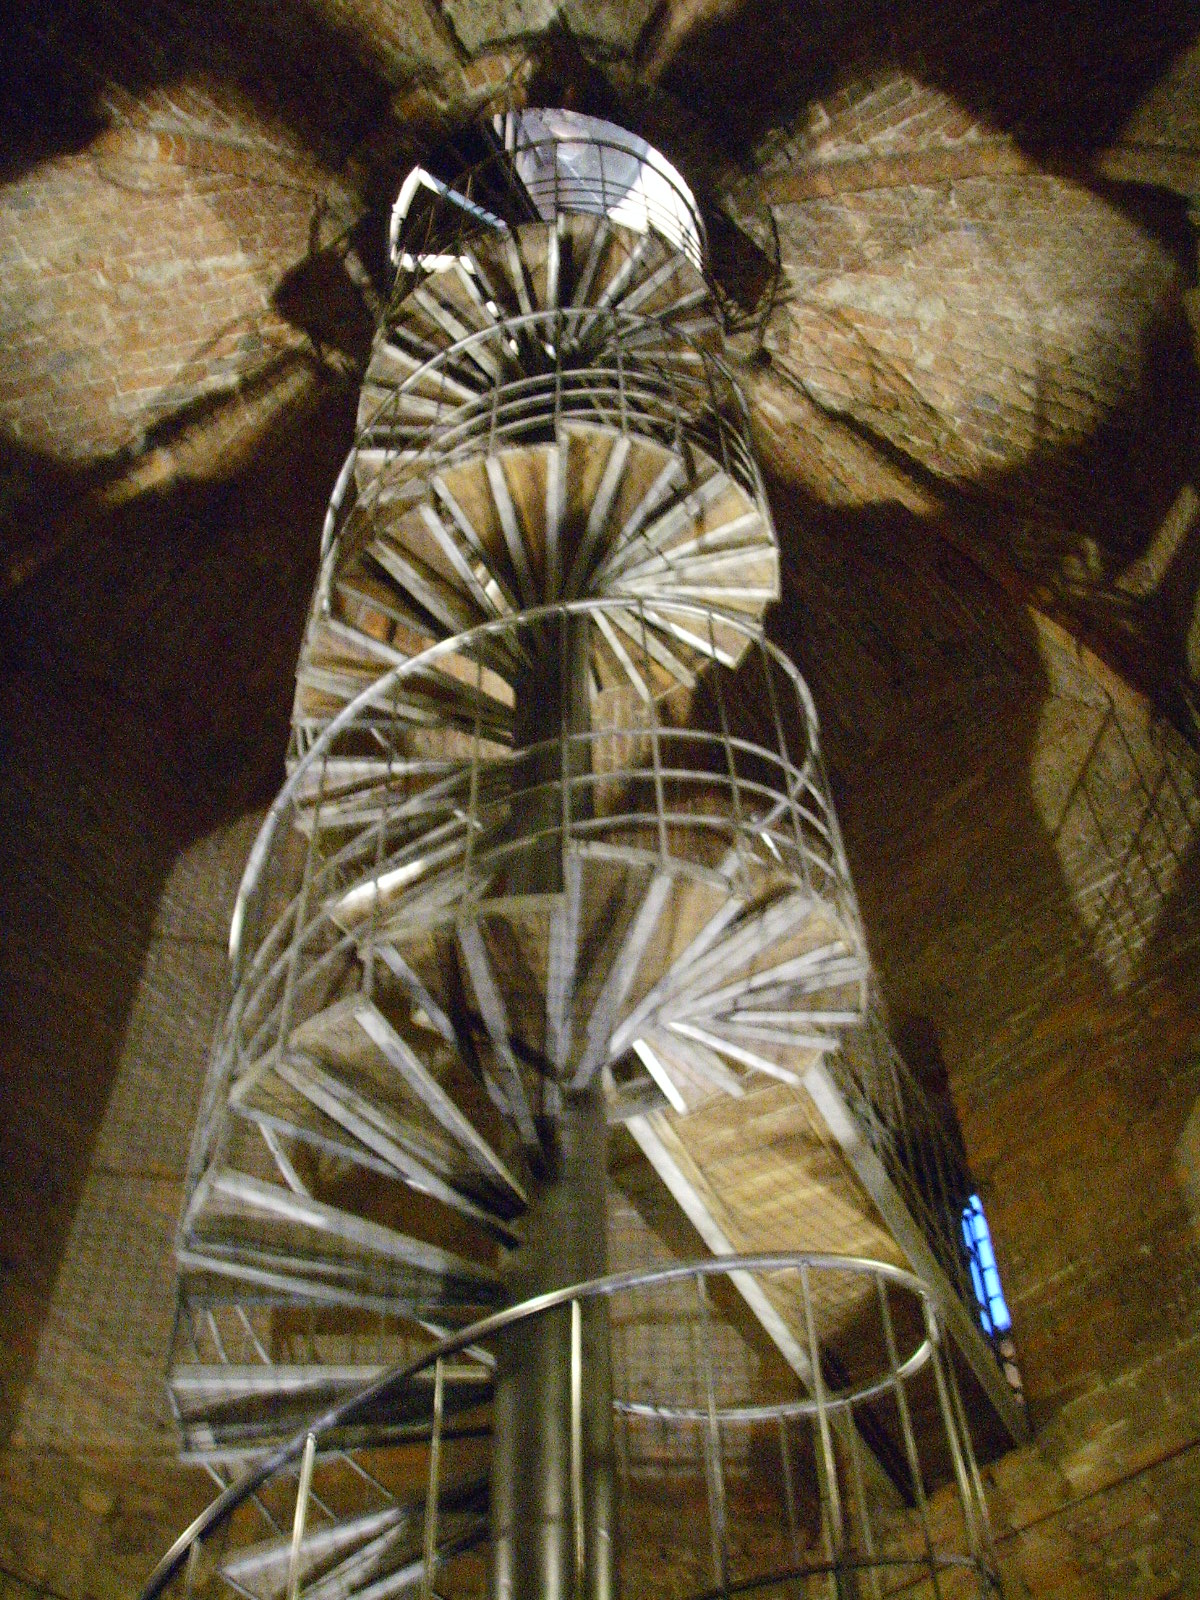
\includegraphics[width=0.35\linewidth]{../Imágenes/Aplicaciones/Cremona,_torrazzo_interno_02_scala_a_chiocciola}
	\caption{Escaleras en el interior de la Torrazzo di Cremona
	\url{http://en.wikipedia.org/wiki/File:Cremona,_torrazzo_interno_02_scala_a_chiocciola.JPG}}
	\label{fig:italia}
\end{figure}

\newpage

\begin{appendices}
\nocite{*}
\bibliographystyle{plain}
\bibliography{../Bibliografía/bibliografia}
\end{appendices}




	
\end{document}